% \documentclass[11pt]{article}
\documentclass[useAMS,usenatbib,referee]{biomweb}
% \usepackage{amssymb, amsthm, amsmath}
\usepackage{amssymb, amsmath}
\usepackage{bm}
\usepackage{graphicx}
% \usepackage[authoryear]{natbib}
\usepackage{bm}
\usepackage{verbatim}
\usepackage{lineno}
\usepackage{times}
\usepackage{soul}
\usepackage{color}
\usepackage{enumitem}
% \usepackage{enumerate}
\usepackage{setspace}
\usepackage{appendix}
% \usepackage{caption}
% \captionsetup[table]{name=Web Table}

% cross-referencing appendices
\usepackage{xr}
\externaldocument{skewt_rev}

% \usepackage[left=1in,top=1in,right=1in]{geometry}
% \pdfpageheight 11in
% \pdfpagewidth 8.5in
% \linespread{2.0}
\newcommand{\btheta}{ \mbox{\boldmath $\theta$}}
\newcommand{\bmu}{ \mbox{\boldmath $\mu$}}
\newcommand{\balpha}{ \mbox{\boldmath $\alpha$}}
\newcommand{\bbeta}{ \mbox{\boldmath $\beta$}}
\newcommand{\bdelta}{ \mbox{\boldmath $\delta$}}
\newcommand{\blambda}{ \mbox{\boldmath $\lambda$}}
\newcommand{\bgamma}{ \mbox{\boldmath $\gamma$}}
\newcommand{\brho}{ \mbox{\boldmath $\rho$}}
\newcommand{\bpsi}{ \mbox{\boldmath $\psi$}}
\newcommand{\bepsilon}{ \mbox{\boldmath $\epsilon$}}
\newcommand{\bomega}{ \mbox{\boldmath $\omega$}}
\newcommand{\bOmega}{ \mbox{\boldmath $\Omega$}}
\newcommand{\bDelta}{ \mbox{\boldmath $\Delta$}}
\newcommand{\bSigma}{ \mbox{\boldmath $\Sigma$}}
\newcommand{\bPsi}{\mbox{\boldmath $\Psi$}}
\newcommand{\bOne}{\mbox{\boldmath $1$}}
\newcommand{\omu}{\overline{\mu}}
\newcommand{\oSigma}{\overline{\Sigma}}
\newcommand{\Yt}{{\tilde Y}}
\newcommand{\bA}{ \mbox{\bf A}}
\newcommand{\bP}{ \mbox{\bf P}}
\newcommand{\bx}{ \mbox{\bf x}}
\newcommand{\bX}{ \mbox{\bf X}}
\newcommand{\bB}{ \mbox{\bf B}}
\newcommand{\bZ}{ \mbox{\bf Z}}
\newcommand{\by}{ \mbox{\bf y}}
\newcommand{\bY}{ \mbox{\bf Y}}
\newcommand{\bz}{ \mbox{\bf z}}
\newcommand{\bh}{ \mbox{\bf h}}
\newcommand{\br}{ \mbox{\bf r}}
\newcommand{\bt}{ \mbox{\bf t}}
\newcommand{\bs}{ \mbox{\bf s}}
\newcommand{\bb}{ \mbox{\bf b}}
\newcommand{\bL}{ \mbox{\bf L}}
\newcommand{\bu}{ \mbox{\bf u}}
\newcommand{\bv}{ \mbox{\bf v}}
\newcommand{\bV}{ \mbox{\bf V}}
\newcommand{\bW}{ \mbox{\bf W}}
\newcommand{\bG}{ \mbox{\bf G}}
\newcommand{\bH}{ \mbox{\bf H}}
\newcommand{\bw}{ \mbox{\bf w}}
\newcommand{\bo}{ \mbox{\bf o}}
\newcommand{\bfe}{ \mbox{\bf e}}
\newcommand{\iid}{\stackrel{iid}{\sim}}
\newcommand{\indep}{\stackrel{indep}{\sim}}
\newcommand{\calR}{{\cal R}}
\newcommand{\calG}{{\cal G}}
\newcommand{\calD}{{\cal D}}
\newcommand{\calS}{{\cal S}}
\newcommand{\calB}{{\cal B}}
\newcommand{\calA}{{\cal A}}
\newcommand{\calT}{{\cal T}}
\newcommand{\calO}{{\cal O}}
\newcommand{\argmax}{{\mathop{\rm arg\, max}}}
\newcommand{\argmin}{{\mathop{\rm arg\, min}}}
\newcommand{\Frechet}{\mbox{Fr$\acute{\mbox{e}}$chet }}
\newcommand{\Matern}{\mbox{Mat$\acute{\mbox{e}}$rn }}
\newcommand{\ballunion}{B_a(\bs_1) \cup B_b(\bs_2) }

\newcommand{\beq}{ \begin{equation}}
\newcommand{\eeq}{ \end{equation}}
\newcommand{\beqn}{ \begin{eqnarray}}
\newcommand{\eeqn}{ \end{eqnarray}}
\renewcommand{\fref}[1]{Web Figure~\ref{#1}}

\title[Web-based Supplementary Materials for A Space-time \Skewt Model for Threshold Exceedances]{Web-based Supplementary Materials for A Space-time \Skewt Model for Threshold Exceedances by Morris, Reich, Thibaud, and Cooley}
\author
{Samuel A Morris$^{1,*}$\email{samorris@ncsu.edu},
Brian J Reich$^{1}$,
Emeric Thibaud$^{2}$, and
Daniel Cooley$^{2}$\\
$^{1}$Department of Statistics, North Carolina State University, Raleigh, North Carolina, U.S.A. \\
$^{2}$Department of Statistics, Colorado State University, Fort Collins, Colorado, U.S.A.}

\begin{document} %\linenumbers
\maketitle
% \begin{center}
% {\Large {\bf Supplemental material for A space-time \skewt model for threshold exceedances}}\\

% {\large Samuel A Morris\footnote[1]{North Carolina State University}, Brian J Reich\footnotemark[1]{}, Emeric Thibaud\footnote[2]{Colorado State University}, and Daniel Cooley\footnotemark[2]{}}

% \today
% \end{center}

% \appendix
\renewcommand{\thesection}{Web Appendix~\Alph{section}}
% \renewcommand{\tablename}{Web Table}
% \renewcommand{\figurename}{Web Figure}
% \renewcommand{\thetable}{Web Table \arabic{table}}

\section{MCMC details} \label{sta:mcmc}
The MCMC sampling for the model in \sref{sts:hier} is done using {\tt R} (http://www.r-project.org). Whenever possible, we select conjugate priors (see \aref{sta:posterior}); however, for some of the parameters, no conjugate prior distributions exist.
For these parameters, we use a random walk Metropolis-Hastings update step.
In each Metropolis-Hastings update, we tune the algorithm during the burn-in period to give acceptance rates near 0.40.

\subsection*{Spatial knot locations}
For each day, we update the spatial knot locations, $\bw_1, \ldots, \bw_K$, using a Metropolis-Hastings block update.
Because the spatial domain is bounded, we generate candidate knots using the transformed knots $\bw^*_1, \ldots, \bw^*_K$ (see \sref{sts:temporal}) and a random walk bivariate Gaussian candidate distribution
\begin{align*}
	{\bw^*_k}^{(c)} \sim \text{N}({\bw^*_k}^{(r - 1)}, s^2 I_2)
\end{align*}
where ${\bw^*_k}^{(r - 1)}$ is the location for the transformed knot at MCMC iteration $r - 1$, $s$ is a tuning parameter, and $I_2$ is an identity matrix.
Let $\bY_t = [Y(\bs_1), \ldots, Y(\bs_n)]$ be the vector of observed responses at each site for day $t$.
After candidates have been generated for all $K$ knots, the acceptance ratio is
\begin{align*}
  R = \left\{ \frac{ l[ \bY_t | \bw_1^{(c)}, \ldots, \bw_K^{(c)}, \ldots] }{l[ \bY_t | \bw_1^{(r - 1)}, \ldots, \bw_K^{(r - 1)}, \ldots]} \right\} \times \left\{ \frac{ \prod_{k = 1}^{K}\phi(\bw_k^{(c)})}{ \prod_{k = 1}^{K}\phi(\bw_k^{(r - 1)})} \right\} \times \left\{ \frac{ \prod_{k = 1}^{K} p({\bw^*_k}^{(c)})}{ \prod_{k = 1}^{K} p({\bw^*_k}^{(r - 1)})}\right\}
\end{align*}
where $l$ is the likelihood given in \eref{steq:hier}, and $p(\cdot)$ is the prior either taken from the time series (see \sref{sts:temporal}) or assumed to be uniform over $\calD$.
The candidate knots are accepted with probability $\min\{R, 1\}$.

\subsection*{Spatial random effects}
If there is no temporal dependence amongst the observations, we use a Gibbs update for $z_{tk}$, and the posterior distribution is given in \aref{sta:posterior}.
If there is temporal dependence amongst the observations, then we update $z_{tk}$ using a Metropolis-Hastings update.
Because this model uses $|z_{tk}|$, we generate candidate random effects using the $z^*_{tk}$ (see \sref{sts:temporal}) and a random walk Gaussian candidate distribution
\begin{align*}
  {z^*_{tk}}^{(c)} \sim \text{N}({z^*_{tk}}^{(r - 1)}, s^2)
\end{align*}
where ${z^*_{tk}}^{(r-1)}$ is the value at MCMC iteration $r - 1$, and $s$ is a tuning parameter.
The acceptance ratio is
\begin{align*}
  R = \left\{ \frac{ l[\bY_t | z_{tk}^{(c)}, \ldots] }{ l[\bY_t | z_{tk}^{(r - 1)}]} \right\} \times \left\{ \frac{ p[ z_{tk}^{(c)} ] }{ p[ z_{tk}^{(r - 1)}]}\right\}
\end{align*}
where $p[\cdot]$ is the prior taken from the time series given in \sref{sts:temporal}.
The candidate is accepted with probability $\min\{R, 1\}$.

\subsection*{Variance terms}
When there is more than one site in a partition, then we update $\sigma^2_{tk}$ using a Metropolis-Hastings update.
First, we generate a candidate for $\sigma^2_{tk}$ using an IG$(a^*/s, b^*/s)$ candidate distribution in an independence Metropolis-Hastings update where $a^* = (n_{tk} + 1) / 2 + a$, $b^* = [\bY_{tk}^\top \Sigma^{-1}_{tk} \bY_{tk} + z_{tk}^2] / 2 + b$, $n_{tk}$ is the number of sites in partition $k$ on day $t$, and $\bY_{tk}$ and $\Sigma^{-1}_{tk}$ are the observations and precision matrix for partition $k$ on day $t$.
The acceptance ratio is
\begin{align*}
  R = \left\{
    \frac{ l[\bY_t | {\sigma^2_{tk}}^{(c)}, \ldots] }
         { l[\bY_t | {\sigma^2_{tk}}^{(r - 1)}]}
    \right\} \times \left\{
    \frac{ l[z_{tk} | {\sigma^2_{tk}}^{(c)}, \ldots] }
         { l[z_{tk} | {\sigma^2_{tk}}^{(r - 1)}, \ldots] }
    \right\} \times \left\{
    \frac{ p[ {\sigma^2_{tk}}^{(c)} ] }
         { p[ {\sigma^2_{tk}}^{(r - 1)}] }
    \right\} \times \left\{
    \frac{ c[ {\sigma^2_{tk}}^{(r - 1)}] }
         { c[ {\sigma^2_{tk}}^{(c)}]}
    \right\}
\end{align*}
where $p[\cdot]$ is the prior either taken from the time series given in \sref{sts:temporal} or assumed to be IG$(a, b)$, and $c[\cdot]$ is the candidate distribution.
The candidate is accepted with probability $\min\{R, 1\}$.

\subsection*{Spatial covariance parameters}
We update the three spatial covariance parameters, $\log(\rho)$, $\log(\nu)$, $\gamma$, using a Metropolis-Hastings block update step.
First, we generate a candidate using a random walk Gaussian candidate distribution
\begin{align*}
	\log(\rho)^{(c)} \sim \text{N}(\log(\rho)^{(r - 1)}, s^2)
\end{align*}
where $\log(\rho)^{(r-1)}$ is the value at MCMC iteration $r - 1$, and $s$ is a tuning parameter.
Candidates are generated for $\log(\nu)$ and $\gamma$ in a similar fashion.
The acceptance ratio is
\begin{align*}
	R = \left\{ \frac{ \prod_{t = 1}^{n_t} l[Y_t(\bs) | \rho^{(c)}, \nu^{(c)}, \gamma^{(c)}, \ldots] }{\prod_{t = 1}^{n_t} l[Y_t(\bs) | \rho^{(r-1)}, \nu^{(r-1)}, \gamma^{(r-1)}, \ldots] } \right\} \times \left\{ \frac{ p[\rho^{(c)}] }{ p[\rho^{(r - 1)] } } \right\} \times \left\{ \frac{ p[\nu^{(c)}] }{ p[\nu^{(r - 1)}] } \right\} \times \left\{ \frac{ p[ \gamma^{(c)} ] }{ p[\gamma^{(r - 1)} ] } \right\}.
\end{align*}
All three candidates are accepted with probability $\min\{R, 1\}$.

\section{Posterior distributions} \label{sta:posterior}

\subsection*{Conditional posterior of $z_{tk} \mid \ldots $}\label{sts:mvcondu}
If knots are independent over days, then the conditional posterior distribution of $|z_{tk}|$ is conjugate.
For simplicity, drop the subscript $t$, let $\tilde{z}_{k} = |z_{k}|$, $\tilde{\bz}_{k^c}$ be the vector of $[|z(\bs_1)|, \ldots, |z(\bs_n)|]$ for $\bs \notin P_k$, $\bX = [\bX(\bs_1), \ldots, \bX(\bs_n)]^\top$, let $\bY_k$ and $\bX_k$ be the observations and covariate measurements for $\bs \in P_k$, and let $\bY_{k^c}$ and $\bX_{k^c}$ be the observations and covariate measurements for $\bs \notin P_k$ and define
\begin{align*}
\bR = \left\{
    \begin{array}{ll}
        \bY_k - \bX_k \bbeta & \bs \in P_k\\[1em]
        \bY_{k^c} - \bX_{k^c} \bbeta - \lambda \tilde{\bz}_{k^c} \qquad & \bs \notin P_k
    \end{array}
\right.
\end{align*}
Let
\begin{align*}
    \bR_1 &= \text{the vector of } \bR \text{ for } \bs \in P_k \\
    \bR_2 &= \text{the vector of } \bR \text{ for } \bs \notin P_k \\
    \Omega &= \Sigma^{-1}.
\end{align*}
Then
\begin{align*}
    \pi(z_k | \ldots) &\propto \exp \left\{ -\frac{ 1 }{ 2 } \left[
        \left( \begin{array}{c}
            \bR_1 - \lambda \tilde{z}_k \bOne\\
            \bR_2
        \end{array} \right)^\top
        \left( \begin{array}{cc}
            \Omega_{11} & \Omega_{12}\\
            \Omega_{21} & \Omega_{22}
        \end{array} \right)
        \left( \begin{array}{c}
            \bR_1 - \lambda \tilde{z}_k \bOne\\
            \bR_2
        \end{array} \right)
        +  \frac{ {\tilde{z}_k}^2 }{ \sigma_k^2 }\right]
    \right\} I(z_k > 0) \\
        &\propto \exp \left\{ -\frac{ 1 }{ 2 } \left[ \Lambda_k {\tilde{z}_k}^2 - 2 \mu_k \tilde{z}_k \right] \right\}
\end{align*}
where
\begin{align*}
    \mu_k &= \lambda ( \bR_1^\top \Omega_{11} + \bR_2^\top \Omega_{21} )\bOne\\
    \Lambda_k &= \lambda^2 \bOne^\top \Omega_{11} \bOne + \frac{ 1 }{ \sigma^2_k }.
\end{align*}
Then $\tilde{z}_k | \ldots \sim N_{(0, \infty)} (\Lambda_k^{-1} \mu_k, \Lambda_k^{-1})$

\subsection*{Conditional posterior of $\bbeta, \lambda \mid \ldots$}\label{sts:betapost}
For models that do not include a skewness parameter, we update $\bbeta$ as follows.
Let $\bbeta \sim \mbox{N}_{p}(0, \Lambda_0)$ where $\Lambda_0$ is a precision matrix.
Then
\begin{align*}
    \pi(\bbeta \mid \ldots) & \propto \exp \left\{ - \frac{ 1 }{ 2 } \bbeta^\top \Lambda_0 \bbeta - \frac{ 1 }{ 2 } \sum_{t = 1}^{n_t} [\bY_t -\bX_t \bbeta]^\top \Omega [\bY_t - \bX_t \bbeta] \right\} \\
     & \propto \exp \left\{ -\frac{ 1 }{ 2 } \left[ \bbeta^\top \Lambda_\beta \bbeta  - 2 \sum_{t = 1}^{n_t} (\bbeta^\top \bX_t^\top \Omega \bY_t) \right] \right\} \\
     & \propto \mbox{N} ( \Lambda_\beta^{-1} \mu_\beta , \Lambda_\beta^{-1})
\end{align*}
where
\begin{align*}
    \mu_\beta &= \sum_{t = 1}^{n_t} \bX_t^\top \Omega \bY_t \\
    \Lambda_\beta &= \Lambda_0 + \sum_{t = 1}^{n_t} \bX_t^\top \Omega \bX_t.
\end{align*}
For models that do include a skewness parameter, a simple augmentation of the covariate matrix $\bX$ and parameter vector $\bbeta$ allows for a block update of both $\bbeta$ and $\lambda$.
Let $\bX^*_{t} = [\bX_t, |\bz_{t}|]$ where $\bz_t = [z(\bs_1), \ldots, z(\bs_{n})]^\top$ and let $\bbeta^* = (\beta_1, \ldots, \beta_p, \lambda)^\top$.
So to incorporate the $N(0, \sigma^2_\lambda)$ prior on $\lambda$, let $\bbeta^* \sim \mbox{N}_{p+1}(0, \Lambda^*_0)$ where
\begin{align*}
  \Lambda^*_0 = \left( \begin{array}{cc}
    \Lambda_0 & 0 \\
    0         & \sigma^{-2}_\lambda
  \end{array}\right).
\end{align*}
Then the update for both $\bbeta$ and $\lambda$ is done using the conjugate prior given above with $\bX_t = \bX_t^*$ and $\bbeta = \bbeta^*$

\subsection*{Conditional posterior of $\sigma^2 \mid \ldots$}\label{sts:sigpost}
In the case where $L = 1$ and temporal dependence is negligible, then $\sigma^2$ has a conjugate posterior distribution.
Let $\sigma_t^2 \iid \mbox{IG}(\alpha_0 / 2, \beta_0 / 2)$. For simplicity, drop the subscript $t$. Then
\begin{align*}
    \pi(\sigma^2 \mid \ldots) & \propto (\sigma^2)^{ -\alpha_0 / 2 - 1 / 2 - n / 2 - 1} \exp \left\{ -\frac{\beta_0}{2\sigma^2} - \frac{ |z|^2 }{2 \sigma^2} - \frac{ (\bY - \bmu)^\top \Sigma^{-1} (\bY - \bmu) }{2 \sigma^2} \right\} \\
    & \propto (\sigma^2)^{ -(\alpha_0 - 1 - n) / 2 - 1} \exp \left\{ - \frac{ 1 }{ 2 \sigma^2 } \left[\beta_0 + |z|^2 + (\bY - \bmu)^\top \Sigma^{-1} (\bY - \bmu) \right] \right\} \\
    & \propto \mbox{IG} (\alpha^*, \beta^*)
\end{align*}
where
\begin{align*}
    \alpha^* &= \frac{\alpha_0 + 1 + n}{2} \\
    \beta^* &= \frac{1}{2} \left[ \beta_0 + |z|^2 + (\bY - \bmu)^\top \Sigma^{-1} (\bY - \bmu) \right].
\end{align*}
In the case that $K > 1$, a random walk Metropolis Hastings step will be used to update $\sigma^2_{kt}$.

\section{Proof that $\lim_{h \rightarrow \infty} \pi(h) = 0$} \label{sta:proofsamepartition}
Let $c$ be the midpoint of $\bs_1$ and $\bs_2$.
Define $A$ as the circle centered at $c$ with radius $h / 2$ where $h = ||\bs_1 - \bs_2||$ is the distance between sites $\bs_1$ and $\bs_2$.
Consider a homogeneous spatial Poisson process over $A$ with intensity $\lambda_{PP}$, so that
\begin{align*}
  \mu_{PP}(A) = \lambda_{PP} |A| = \lambda_{PP} \pi \left(\frac{h}{2}\right)^2 = \lambda_{PPA}^* h^2.
\end{align*}
Consider a partition of $A$ into four regions, $B_1$, $B_2$, $R_1$, $R_2$ as seen in \fref{stfig:hpp}.
\begin{figure}
  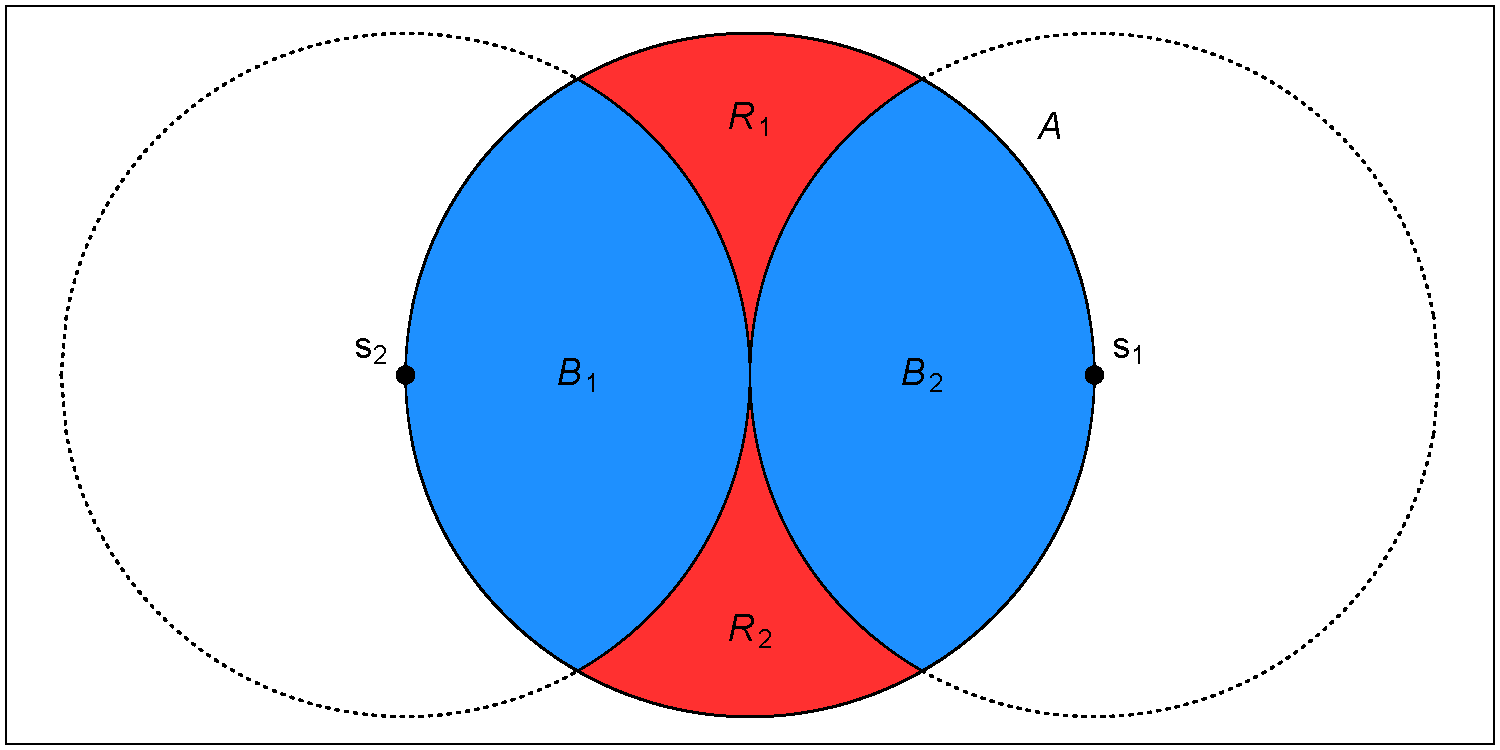
\includegraphics[width=\linewidth]{plots/circles}
  \caption{Illustration of the partition of $A$.}
  \label{stfig:hpp}
\end{figure}
Let $N_i$ be the number of knots in $B_i$ and $L_i = l$ if $\bs_i \in P_l$ for $i = 1, 2$.
Then
\begin{align}
  P(L_1 \neq L_2) \ge P(N_1 > 0, N_2 > 0)
\end{align}
since knots in both $B_1$ and $B_2$ is sufficient, but not necessary, to ensure that $\bs_1$ and $\bs_2$ are in different partition sets.
By definition of a Poission process, $N_1$ and $N_2$ are independent and thus $P(N_1 > 0, N_2 > 0) = P(N_1 > 0)^2$, and
\begin{align}
  \mu_{PP}(B_1) &= \lambda_{PP} |B_1| = \lambda_{PP} \frac{h^2}{4} \left(\frac{2 \pi}{3} - \frac{\sqrt{3}}{2} \right) \nonumber \\
       &= \lambda^*_{PPB1} h^2.
\end{align}
So,
\begin{align}
  P(L_1 \neq L_2) >= P(N_1 > 0)^2 = [1 - P(N_1 = 0)]^2 = [1 - \exp\left(-\lambda^*_{PPB1} h^2\right)]^2
\end{align}
which goes to 1 as $h$ goes to infinity.

%Then $\bs_1$ and $\bs_2$ are in different partitions almost surely if two or more points are in $A$.
%Let $N(A)$ be the number of points in $A$, and let
%\begin{align*}
%  \mu(A) = \lambda_{PP} |A| = \lambda_{PP} \pi \left(\frac{h}{2}\right)^2 = \lambda_{PP}^* h^2.
%\end{align*}

%
%
%Then
%\begin{align*}
%  P[N(A) \ge 2] &= 1 - P[N(A) = 0] - P[N(A) = 1]\\
%                &= 1 - \exp\{-\lambda h^2\} - \lambda h^2 \exp\{-\lambda h^2\} \\
%                &= 1 - (1 + \lambda h^2) \exp\{-\lambda h^2\}
%\end{align*}
%which goes to one as $h \rightarrow \infty$.


% Let $N(A)$ be the number of knots in $A$.
% So,
% \begin{align*}
%   P[ N(A) = k] = \frac{ \mu(A)^k \exp\{ -\mu(A)\}}{k!}.
% \end{align*}
% Then for any finite $k$, $\lim_{h \rightarrow \infty} P[N(A) = k] = 0$ because $\lim_{h \rightarrow \infty} \mu(A) = \infty$.
% With each additional knot in $A$, the chance that $\bs_1$ and $\bs_2$ will be be in the same partition will decrease, because partition membership is defined by the closest knot to a site.
% Therefore, $\lim_{h \rightarrow \infty} \pi(h) = 0$.

% \subsection{Half-normal distribution}
% Let $u = |z|$ where $Z \sim N(\mu, \sigma^2)$.
% Specifically, we consider the case where $\mu = 0$. Then $U$ follows a half-normal distribution which we denote as $U \sim HN(0, 1)$, and the density is given by
% \begin{align}
%   f_U(u) = \frac{ \sqrt{2} }{ \sqrt{\pi \sigma^2} } \exp \left( - \frac{ u^2 }{ 2 \sigma^2 } \right) I(u > 0)
% \end{align}
% When $\mu = 0$, the half-normal distribution is also equivalent to a $N_{(0, \infty)}(0, \sigma^2)$ where $N_{(a, b)}(\mu, \sigma^2)$ represents a normal distribution with mean $\mu$ and standard deviation $\sigma$ that has been truncated below at $a$ and above at $b$.

\section{\Skewt distribution} \label{sta:skewt}
\subsection*{Univariate \skewt distribution}
We say that $Y$ follows a univariate extended \skewt distribution with location $\xi \in \calR$, scale $\omega > 0$, skew parameter $\alpha \in \calR$, and degrees of freedom $\nu$ if has distribution function
\begin{align}
  f_{\text{EST}}(y) = 2 f_T (z; \nu) F_T\left[ \alpha z \sqrt{ \frac{ \nu + 1 }{ \nu + z^2}}; \nu + 1 \right]
\end{align}
where $f_T(t; \nu)$ is a univariate Student's $t$ with $\nu$ degrees of freedom, $F_T(t; \nu) = P(T < t)$, and \hbox{$z = (y - \xi) / \omega$}.

\subsection*{Multivariate \skewt distribution}
If $\bZ \sim \text{ST}_d(0, \bar{\bOmega}, \balpha, \eta)$ is a $d$-dimensional \skewt distribution, and $\bY = \xi + \bomega \bZ$, where $\bomega = \text{diag}(\omega_1, \ldots, \omega_d)$, then the density of $Y$ at $y$ is
\begin{align}
  f_y(\by) = det(\bomega)^{-1} f_z(\bz)
\end{align}
where
\begin{align}
  f_z(\bz) &= 2 t_d(\bz; \bar{\bOmega}, \eta) T \left[ \balpha^\top \bz \sqrt{ \frac{\eta + d}{\nu + Q(\bz)} }; \eta + d\right] \\
  \bz &= \bomega^{-1}(\by - \xi)
\end{align}
where $t_d(\bz; \bar{\bOmega}, \eta)$ is a $d$-dimensional Student's $t$-distribution with scale matrix $\bar{\bOmega}$ and degrees of freedom $\eta$, $Q(z) = \bz^\top \bar{\Omega}^{-1}\bz$ and $T(\cdot; \eta)$ denotes the univariate Student's $t$ distribution function with $\eta$ degrees of freedom \citep{Azzalini2014}.

\subsection*{Extremal dependence}
For a bivariate \skewt random variable $\bY = [Y(\bs), Y(\bt)]^\top$, the $\chi(h)$ statistic \citep{Padoan2011} is given by
\begin{align} \label{steq:chiskew-t}
  \chi(h) = \bar{F}_{\text{EST}}\left\{ \frac{[x_1^{1 / \eta} - \varrho(h)] \sqrt{\eta + 1} }{\sqrt{1 - \varrho(h)^2}}; 0, 1, \alpha_1, \tau_1, \eta + 1 \right\} + \bar{F}_{\text{EST}}\left\{ \frac{ [x_2^{1 / \eta} - \varrho(h)] \sqrt{\eta + 1} }{ \sqrt{1 - \varrho(h)^2} }; 0, 1, \alpha_2, \tau_2, \eta + 1 \right\},
\end{align}
where $\bar{F}_{\text{EST}}$ is the univariate survival extended \skewt function with zero location and unit scale, \hbox{$\varrho(h) = \text{cor}[y(\bs), y(\bt)]$}, $\alpha_j = \alpha_i \sqrt{1 - \varrho^2}$, $\tau_j = \sqrt{\eta + 1}(\alpha_j + \alpha_i \varrho)$, and $x_j = F_T(\bar{\alpha}_i \sqrt{\eta + 1}; 0, 1, \eta) / F_T(\bar{\alpha}_j \sqrt{\eta + 1}; 0, 1, \eta)$ with $j = 1, 2$ and $i = 2, 1$ and where $\bar{\alpha}_j = (\alpha_j + \alpha_i \varrho) / \sqrt{ 1 + \alpha_i^2 [1 - \varrho(h)^2]}$.

\subsection*{Proof that $\lim_{h \rightarrow \infty} \chi(h) > 0$}
Consider the bivariate distribution of $\bY = [Y(\bs), Y(\bt)]^\top$, with $\varrho(h)$ given by \eref{steq:matern}.
So, $\lim_{h \rightarrow \infty} \varrho(h) = 0$.
Then
\begin{align}
  \lim_{h \rightarrow \infty} \chi(h) = \bar{F}_{\text{EST}}\left\{ \sqrt{\eta + 1}; 0, 1, \alpha_1, \tau_1, \eta + 1 \right\} + \bar{F}_{\text{EST}}\left\{ \sqrt{\eta + 1}; 0, 1, \alpha_2, \tau_2, \eta + 1 \right\}.
\end{align}
Because the extended \skewt distribution is not bounded above, for all $\bar{F}_{\text{EST}}(x) = 1 - F_{\text{EST} (x)} > 0$ for all $x < \infty$.
Therefore, for a \skewt distribution, $\lim_{h \rightarrow \infty} \chi(h) > 0$.

\section{Comparisons with other parameterizations} \label{sta:otherparams}
Various forms of multivariate skew-normal and \skewt distributions have been proposed in the literature.
In this section, we make a connection between our parameterization in \eref{steq:fullmodel} of the main text and another popular version.
\citet{Azzalini2014} and \citet{Beranger2016} define a skew-normal process as
\begin{align}
  \tilde{X}(\bs) = \tilde{\lambda}|z| + (1 - \tilde{\lambda}^2)^{1 / 2} v(\bs)
\end{align}
where $\tilde{\lambda} \in (-1, 1)$, $z \sim N(0, 1)$, and $v(\bs)$ is a Gaussian process with mean zero, variance one, and spatial correlation function $\rho$.
To extend this to the \skewt distribution, \citet{Azzalini2003} take $\tilde{Y}(\bs) = W\tilde{X}(\bs)$ where $W^{-2} \sim $ Gamma$(a / 2, a / 2)$.
Returning to the proposed parameterization (with $\bbeta = 0$), let $W^{-2} = \frac{b}{a}\sigma^{-2}$ so that \eref{steq:fullmodel} in the manuscript becomes
\begin{align}
  Y(\bs) = W \left[ \lambda \left(\frac{b}{a}\right)^{1 / 2} |z| + \left(\frac{b}{a}\right)^{1 / 2} v(\bs) \right].
\end{align}
Clearly setting $b / a = (1 - \tilde{\lambda}^2) > 0$, and $\lambda = \tilde{\lambda} / (1 - \tilde{\lambda}^2)^{1 / 2} \in (-\infty, \infty)$ resolves the difference in parameterizations.
We note that our parameterization has three parameters $(a, b, \lambda)$ compared to the two parameters of the alternative parameterization $(a, \tilde{\lambda})$.
Since we have assumed that both $v(\bs)$ and $z$ have unit scale, the additional $b$ parameter in our parameterization is required to control the precision.
% However, if we introduce an overall scale parameter $c > 0$ into the alternative parameterization so that $\tilde{Y}(\bs) = c W \tilde{X}(\bs)$, then the two models remain equivalent by setting $a = \nu$, $b = \frac{\nu}{c^2 (1 - \tilde{\lambda}^2)}$, and $\lambda = \tilde{\lambda} / (1 - \tilde{\lambda}^2)^{1 / 2}$.

\section{Temporal dependence} \label{sta:temporal}
It is very challenging to derive an analytical expression the temporal extremal dependence at a single site $\bs$.
However, using simulated data, we have evidence to suggest that the model does exhibits temporal extremal dependence.
To demonstrate that our model maintains temporal extremal dependence, we generate lag-$m$ observations for $m = 1, 3, 5, 10$ from our model setting $\phi_w = \phi_z = \phi_\sigma = \varphi$, for $\varphi = 0, 0.02, 0.04, \ldots, 1$.
To estimate the lag-$m$ chi-statistic $\chi(m)$ we first estimate the lag-$m$ $F$-madogram $\nu_F(m)$ \citep{Cooley2006} using $\hat{\nu}_F(m) = \frac{1}{2n} \sum_{i = 1}^n | \hat{F}(y_{0}) - \hat{F}(y_{m})|$ where $\hat{F}(\cdot)$ represents an empirical CDF and $y_m$ is the lag-$m$ observation.
The $F$-madogram is related to the $\chi$ statistic as follows
\begin{align}
  \chi = 2 - \frac{1 + 2 \nu_F}{1 - 2 \nu_F}.
\end{align}
\fref{stfig:chiphi} suggests that the extremal dependence increases as $\varphi \rightarrow 1$, and that the extremal dependence decreases as $m$ increases.
\begin{figure}
  \centering
  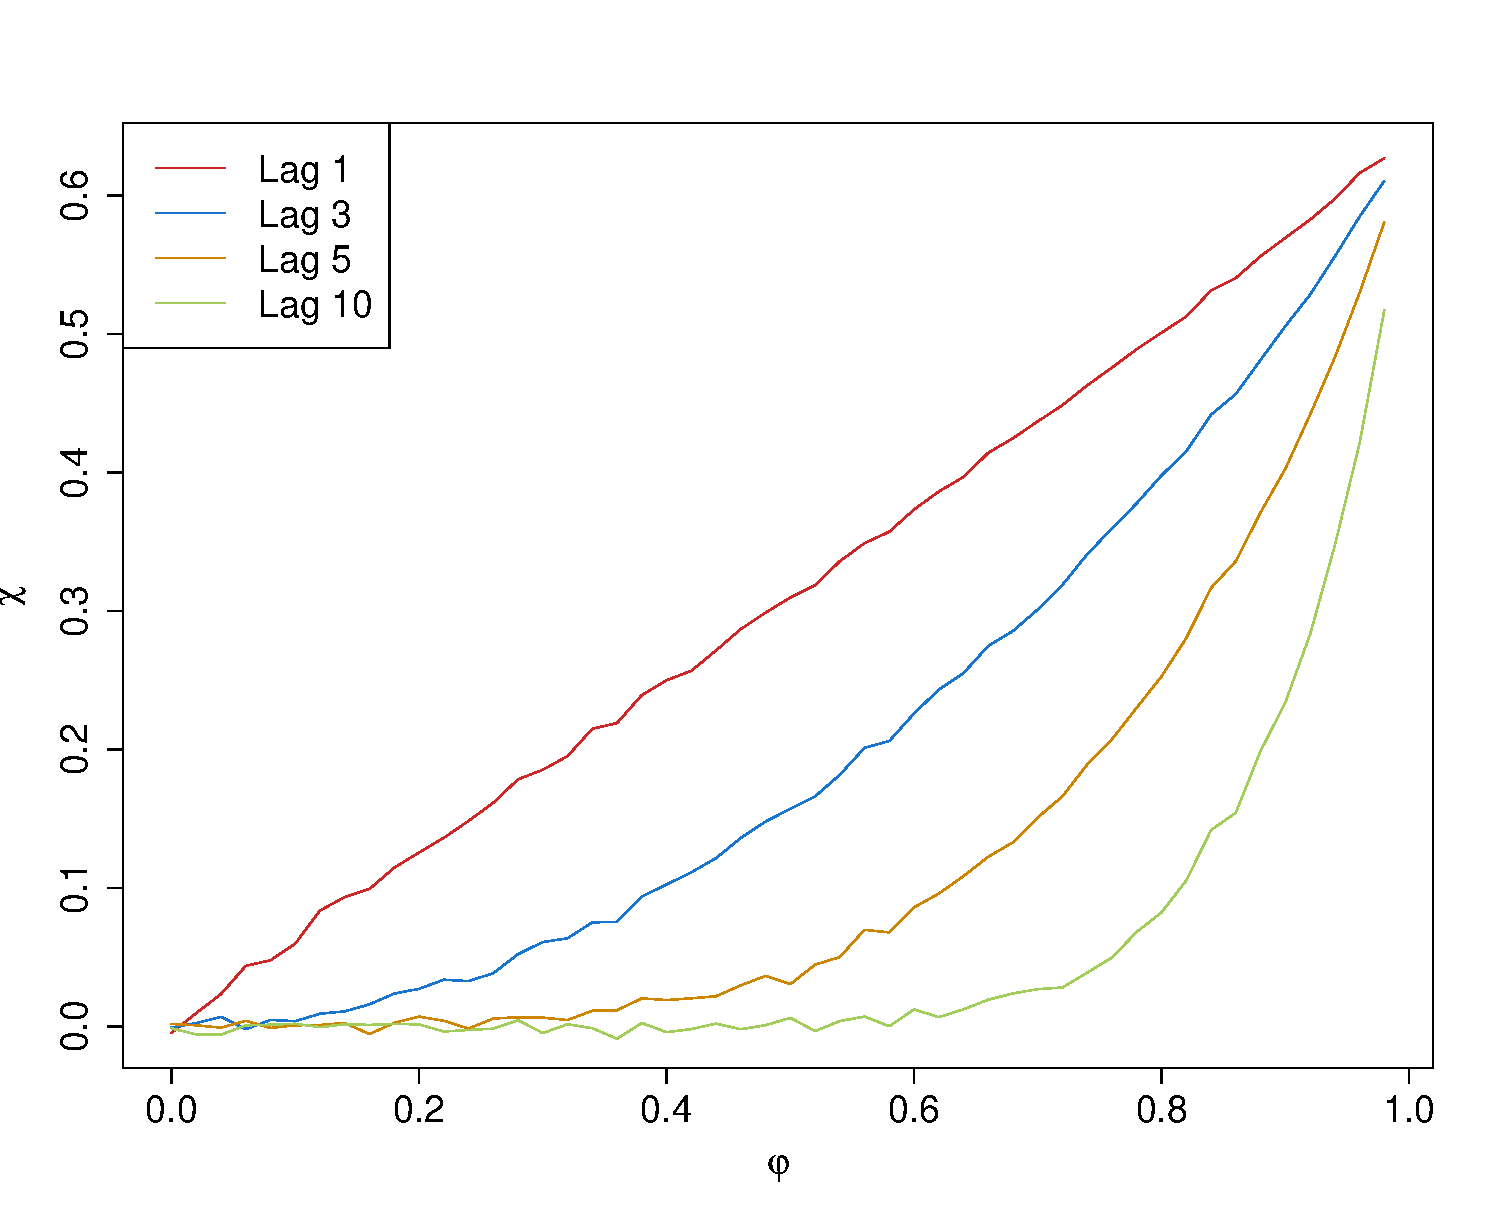
\includegraphics[width=\linewidth]{plots/chi-phi}
  \caption{Simulated lag-$m$ $\chi$ for varying levels of $\varphi$.}
  \label{stfig:chiphi}
\end{figure}

\section{Brier scores for ozone prediction} \label{sta:ozonesite}
Because typical ozone concentration varies throughout the US, we have included Brier scores for exceedance of the 99th quantile by site for two model fits (Gaussian and Symmetric-$t$, $K = $ 10 knots, $T = $ 75, time series) in \fref{stfig:bssite}.
As we can see in these plots, both models seem to perform similarly across the US with the poorest performance in California.
Other methods have similar Brier score maps to these.
\begin{figure}
  \centering
  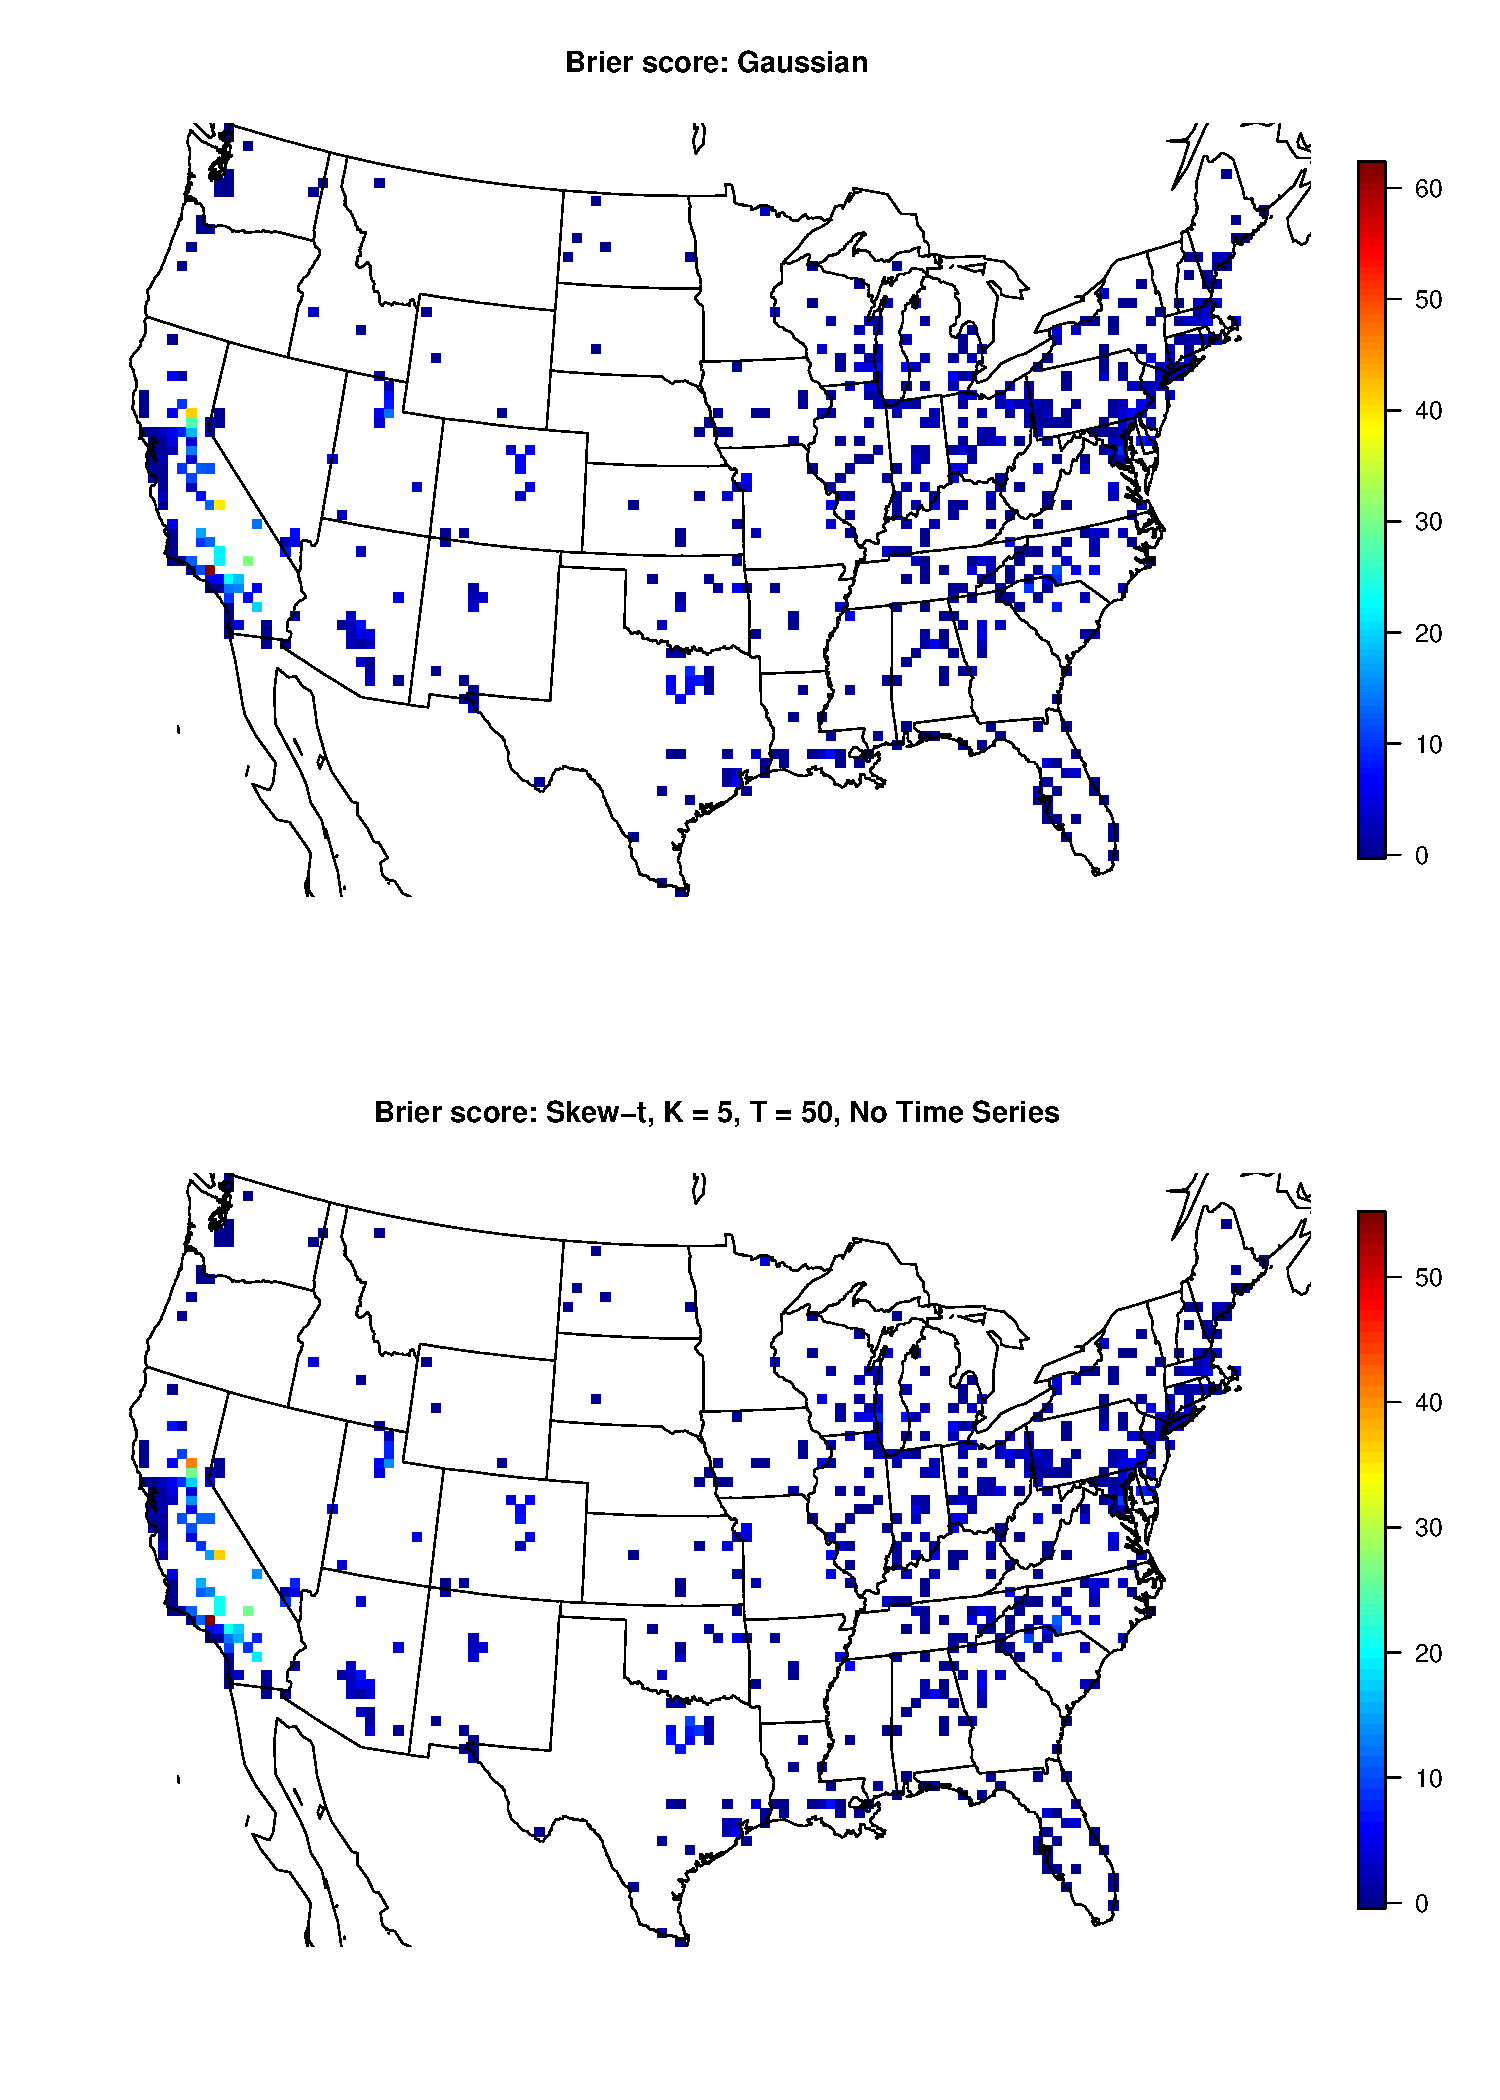
\includegraphics[width=0.8\linewidth]{plots/bs-site}
  \caption{Map of Brier scores for Gaussian (top) vs Symmetric-$t$, $K = $ 10 knots, $T = $ 75, time series (bottom).}
  \label{stfig:bssite}
\end{figure}

\section{Simulation study pairwise difference results} \label{sta:pdiffs}
The following tables show the methods that have significantly different Brier scores when using a Wilcoxon-Nemenyi-McDonald-Thompson test.
In each column, different letters signify that the methods have significantly different Brier scores.
For example, there is significant evidence to suggest that method 1 and method 4 have different Brier scores at $q(0.90)$, whereas there is not significant evidence to suggest that method 1 and method 2 have different Brier scores at $q(0.90)$.
In each table group A represents the group with the lowest Brier scores.
Groups are significant with a familywise error rate of $\alpha = 0.05$.

\begin{table}[htbp]
  \centering
  \caption{Setting 1 -- Gaussian marginal, $K = 1$ knot}
  \label{sttbl:gaussim}
  \begin{tabular}{|l|ccc|ccc|cccc|cc|}
    \cline{2-13}
    \multicolumn{1}{c}{} & \multicolumn{3}{|c}{$q(0.90)$} & \multicolumn{3}{|c}{$q(0.95)$} & \multicolumn{4}{|c}{$q(0.98)$} & \multicolumn{2}{|c|}{$q(0.99)$} \\
    \hline
    Method 1 & A &   &   & A &   &   & A &   &   &   & A &   \\
    \hline
    Method 2 & A &   &   & A &   &   & A &   &   &   & A &   \\
    \hline
    Method 3 &   & B &   &   & B &   &   &   & C &   & A &   \\
    \hline
    Method 4 & A &   &   & A &   &   & A & B &   &   & A &   \\
    \hline
    Method 5 &   & B &   &   & B &   &   & B & C &   & A &   \\
    \hline
    Method 6 &   &   & C &   &   & C &   &   &   & D &   & B \\
    \hline
  \end{tabular}
\end{table}

% \begin{table}[htbp]
%   \centering
%   \caption{Setting 2: Symmetric-$t$ marginal, $K = 1$ knot}
%   \label{tbl:t1k1sim}
%   \begin{tabular}{|l|cc|cccc|cccc|ccc|}
%     \cline{2-14}
%     \multicolumn{1}{c}{} & \multicolumn{2}{|c}{$q(0.90)$} & \multicolumn{4}{|c}{$q(0.95)$} & \multicolumn{4}{|c}{$q(0.98)$} & \multicolumn{3}{|c|}{$q(0.99)$} \\
%     \hline
%     Method 1 &   & B &   &   &   & D &   &   &   & D &   &   & C \\
%     \hline
%     Method 2 & A &   & A &   &   &   & A &   &   &   & A &   &   \\
%     \hline
%     Method 3 &   & B &   & B &   &   &   & B & C &   &   & B &   \\
%     \hline
%     Method 4 & A &   &   &   & C &   &   & B &   &   &   & B &   \\
%     \hline
%     Method 5 &   & B &   &   &   & D &   &   & C & D &   & B & C \\
%     \hline
%   \end{tabular}
% \end{table}

% \begin{table}[htbp]
%   \centering
%   \caption{Setting 3: Symmetric-$t$ marginal, $K = 5$ knots}
%   \label{tbl:gaussim}
%   \begin{tabular}{|l|cc|cc|cc|cc|}
%     \cline{2-9}
%     \multicolumn{1}{c}{} & \multicolumn{2}{|c}{$q(0.90)$} & \multicolumn{2}{|c}{$q(0.95)$} & \multicolumn{2}{|c}{$q(0.98)$} & \multicolumn{2}{|c|}{$q(0.99)$} \\
%     \hline
%     Method 1 &   & B &   & B &   & B &   & B \\
%     \hline
%     Method 2 &   & B &   & B &   & B &   & B \\
%     \hline
%     Method 3 &   & B &   & B &   & B & A & B \\
%     \hline
%     Method 4 & A &   & A &   & A &   & A &   \\
%     \hline
%     Method 5 &   & B &   & B & A & B & A & B \\
%     \hline
%   \end{tabular}
% \end{table}

\begin{table}[htbp]
  \centering
  \caption{Setting 2 -- \Skewt marginal, $K = 1$ knot}
  \label{sttbl:st1sim}
  \begin{tabular}{|l|cccc|cccc|cccc|ccc|}
    \cline{2-16}
    \multicolumn{1}{c}{} & \multicolumn{4}{|c}{$q(0.90)$} & \multicolumn{4}{|c}{$q(0.95)$} & \multicolumn{4}{|c}{$q(0.98)$} & \multicolumn{3}{|c|}{$q(0.99)$} \\
    \hline
    Method 1 &   & B &   &   &   & B &   &   &   & B &   &   &   & B &   \\
    \hline
    Method 2 & A &   &   &   & A &   &   &   & A &   &   &   & A &   &   \\
    \hline
    Method 3 & A & B &   &   & A & B &   &   & A & B &   &   & A & B &   \\
    \hline
    Method 4 & A & B &   &   & A & B &   &   & A & B &   &   & A & B &   \\
    \hline
    Method 5 &   &   & C &   &   &   & C &   &   &   & C &   &   &   & C \\
    \hline
    Method 6 &   &   &   & D &   &   &   & D &   &   &   & D &   &   & C \\
    \hline
  \end{tabular}
\end{table}

\begin{table}[htbp]
  \centering
  \caption{Setting 3 -- \Skewt marginal, $K = 5$ knots}
  \label{sttbl:st5sim}
  \begin{tabular}{|l|cccc|cccc|ccc|ccc|}
    \cline{2-15}
    \multicolumn{1}{c}{} & \multicolumn{4}{|c}{$q(0.90)$} & \multicolumn{4}{|c}{$q(0.95)$} & \multicolumn{3}{|c}{$q(0.98)$} & \multicolumn{3}{|c|}{$q(0.99)$} \\
    \hline
    Method 1 &   &   & C &   &   &   & C &   &   & B &   &   & B &   \\
    \hline
    Method 2 &   &   & C &   &   &   & C &   &   & B &   &   & B &   \\
    \hline
    Method 3 &   & B &   &   &   & B &   &   & A &   &   & A &   &   \\
    \hline
    Method 4 & A &   &   &   & A &   &   &   & A &   &   & A &   &   \\
    \hline
    Method 5 & A &   &   &   & A &   &   &   & A &   &   & A &   &   \\
    \hline
    Method 6 &   &   &   & D &   &   &   & D &   &   & C &   &   & C \\
    \hline
  \end{tabular}
\end{table}

\begin{table}[htbp]
  \centering
  \caption{Setting 4 -- Max-stable, Asymmetric logistic}
  \label{sttbl:mssim}
  \begin{tabular}{|l|cccc|cccc|ccc|ccc|}
    \cline{2-15}
    \multicolumn{1}{c}{} & \multicolumn{4}{|c}{$q(0.90)$} & \multicolumn{4}{|c}{$q(0.95)$} & \multicolumn{3}{|c}{$q(0.98)$} & \multicolumn{3}{|c|}{$q(0.99)$} \\
    \hline
    Method 1 & A & B &   &   &   & B &   &   &   & B &   &   &   & C \\
    \hline
    Method 2 &   & B &   &   &   & B &   &   &   & B &   &   & B & C \\
    \hline
    Method 3 &   &   & C & D &   &   & C &   &   & B &   &   & B &   \\
    \hline
    Method 4 &   &   &   & D &   &   &   & D &   &   & C &   &   & C \\
    \hline
    Method 5 &   &   & C &   &   & B & C &   &   & B &   &   & B & C \\
    \hline
    Method 6 & A &   &   &   & A &   &   &   & A &   &   & A &   &   \\
    \hline
  \end{tabular}
\end{table}

\begin{table}[htbp]
  \centering
  \caption{Setting 5 -- Max-stable, Brown-Resnick}
  \label{sttbl:transsim}
  \begin{tabular}{|l|cccc|ccc|ccc|ccc|}
    \cline{2-14}
    \multicolumn{1}{c}{} & \multicolumn{4}{|c}{$q(0.90)$} & \multicolumn{3}{|c}{$q(0.95)$} & \multicolumn{3}{|c}{$q(0.98)$} & \multicolumn{3}{|c|}{$q(0.99)$} \\
    \hline
    Method 1 &   &   &   & D &   &   & C &   &   & C &   &   & C \\
    \hline
    Method 2 &   &   &   & D &   &   & C &   &   & C &   &   & C \\
    \hline
    Method 3 & A & B &   &   & A &   &   & A & B &   &   & B &   \\
    \hline
    Method 4 &   &   & C &   &   & B &   &   & B &   &   & B &   \\
    \hline
    Method 5 & A &   &   &   & A &   &   & A &   &   & A & B &   \\
    \hline
    Method 6 &   & B & C &   & A &   &   & A &   &   & A &   &   \\
    \hline
  \end{tabular}
\end{table}

% \begin{singlespace}
\bibliographystyle{biom}
\bibliography{library}
% \end{singlespace}

\end{document}

